\newSec[MusterBridge]{Brücke}{3}

DroneController\_pkg zu parrot\_pkg







\glqq Eigentlich basiert jede Dependency Inversion auf einer Brücke\grqq




\newSec{Klassifikation}{4}




\newSec{Struktur und beteiligte Akteure}{4}

\begin{figure}[ht!]
\vspace{0.25cm}
\begin{center}
\fbox{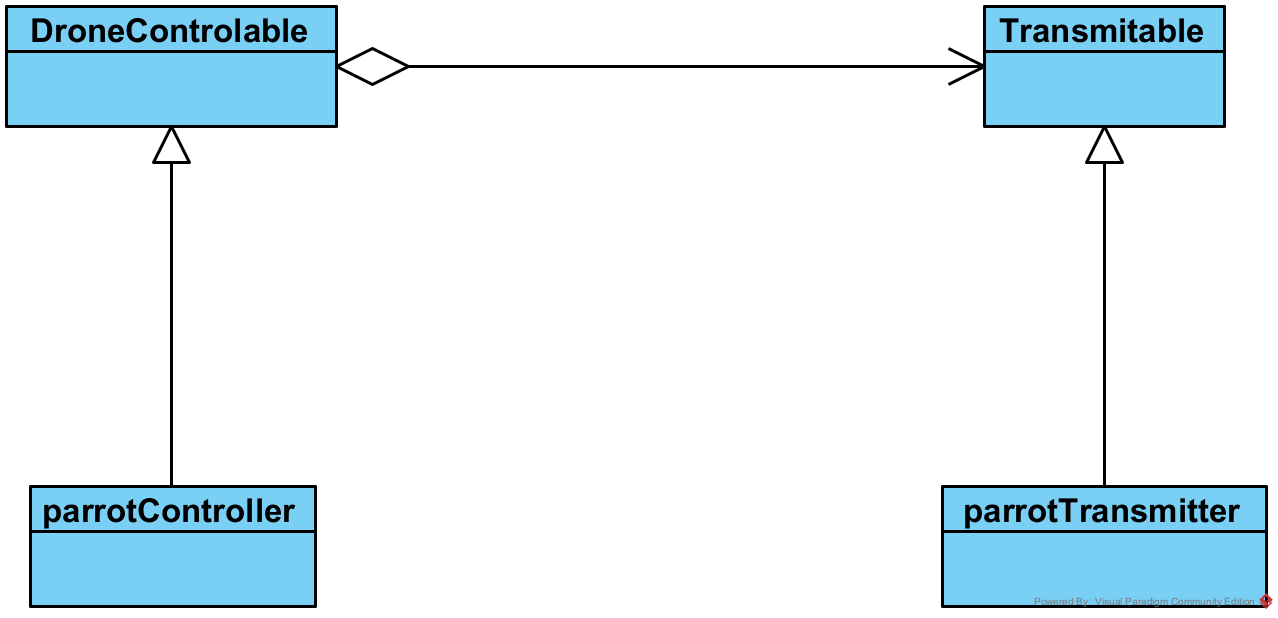
\includegraphics[width=15cm]{Pictures/Bridge.png}}
\caption{Brücke im Projekt}
\label{fig:Bridge}
\end{center}

\vspace{0.25cm}
\refImgShort{fig:Bridge} zeigt \missing\
\end{figure}



\newSec{Motivation}{4}
Das ist eine Design-Entscheidung um im weiteren Lebenszyklus der \textit{Application} verschiedene Dronen als \textit{PlugIn} einbinden zu können.











